در این پوشه رابط تعامل کاربر با سیستم انجام می‌شود.

\begin{figure}[H]
	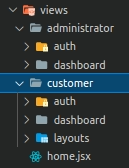
\includegraphics[width=.3\textwidth]{Folders-Files/views.png}
	\centering
	\caption{ساختار پوشه نما}
	\label{fig:folder-views}
\end{figure}


\paragraph{پوشه administrator}
در این پوشه به قالب مدیریت پرداخته شده است.

\paragraph{پوشه customer}
در این پوشه به قالب کاربر که شامل کارفرما و فریلنسر پرداخته شده است.

\subparagraph{پوشه auth}
در این پوشه به قالب احرازهویت کاربر پرداخته شده است.

\subparagraph{پوشه dashboard}
در این پوشه به قالب داشبوردهای کارفرما و فریلنسر پرداخته شده است.

\subparagraph{پوشه employer}
در این پوشه به اجرای قالب داشبورد کارفرما پرداخته شده است.

\subparagraph{پوشه frelanser}
در این پوشه به اجرای قالب داشبورد فریلنسر پرداخته شده است.

\subparagraph{پوشه component}
در این پوشه به قالب‌های پویا مانند باکس‌ها، نمودارها، اعلانات و ... پرداخته شده است.
\subparagraph{پوشه layouts}
در این پوشه به قالب تکرارشونده مانند منوها، هدر، فوتر و ... پرداخته شده است.